% Created by tikzDevice version 0.12.3 on 2020-04-05 20:07:00
% !TEX encoding = UTF-8 Unicode
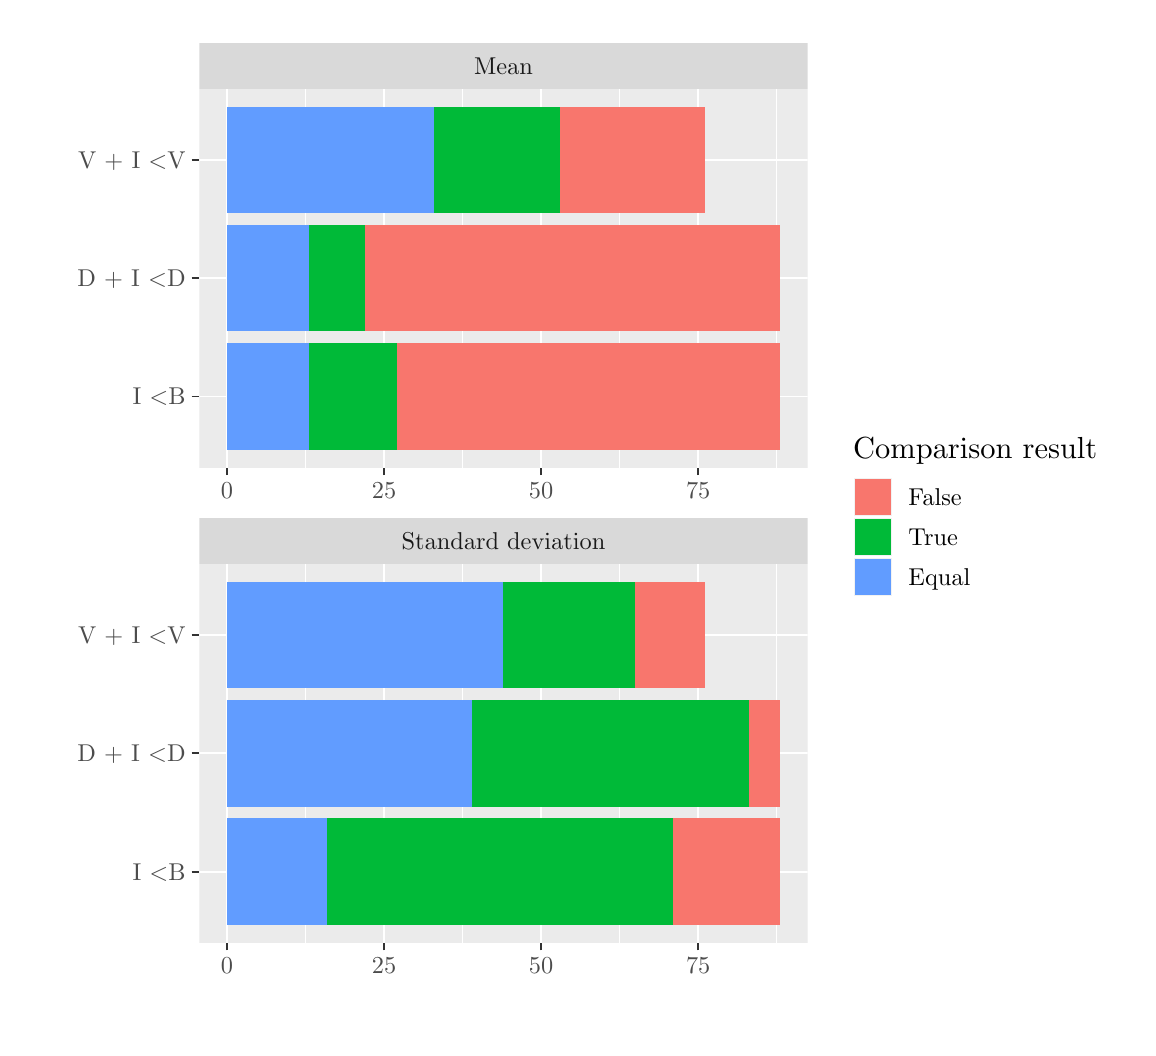
\begin{tikzpicture}[x=1pt,y=1pt]
\definecolor{fillColor}{RGB}{255,255,255}
\path[use as bounding box,fill=fillColor,fill opacity=0.00] (0,0) rectangle (397.48,361.35);
\begin{scope}
\path[clip] (  0.00,  0.00) rectangle (397.48,361.35);
\definecolor{drawColor}{RGB}{255,255,255}
\definecolor{fillColor}{RGB}{255,255,255}

\path[draw=drawColor,line width= 0.6pt,line join=round,line cap=round,fill=fillColor] (  0.00,  0.00) rectangle (397.48,361.35);
\end{scope}
\begin{scope}
\path[clip] ( 62.02,202.38) rectangle (281.82,339.28);
\definecolor{fillColor}{gray}{0.92}

\path[fill=fillColor] ( 62.02,202.38) rectangle (281.82,339.28);
\definecolor{drawColor}{RGB}{255,255,255}

\path[draw=drawColor,line width= 0.3pt,line join=round] (100.39,202.38) --
	(100.39,339.28);

\path[draw=drawColor,line width= 0.3pt,line join=round] (157.16,202.38) --
	(157.16,339.28);

\path[draw=drawColor,line width= 0.3pt,line join=round] (213.93,202.38) --
	(213.93,339.28);

\path[draw=drawColor,line width= 0.3pt,line join=round] (270.70,202.38) --
	(270.70,339.28);

\path[draw=drawColor,line width= 0.6pt,line join=round] ( 62.02,228.05) --
	(281.82,228.05);

\path[draw=drawColor,line width= 0.6pt,line join=round] ( 62.02,270.83) --
	(281.82,270.83);

\path[draw=drawColor,line width= 0.6pt,line join=round] ( 62.02,313.61) --
	(281.82,313.61);

\path[draw=drawColor,line width= 0.6pt,line join=round] ( 72.01,202.38) --
	( 72.01,339.28);

\path[draw=drawColor,line width= 0.6pt,line join=round] (128.78,202.38) --
	(128.78,339.28);

\path[draw=drawColor,line width= 0.6pt,line join=round] (185.54,202.38) --
	(185.54,339.28);

\path[draw=drawColor,line width= 0.6pt,line join=round] (242.31,202.38) --
	(242.31,339.28);
\definecolor{fillColor}{RGB}{97,156,255}

\path[fill=fillColor] ( 72.01,208.80) rectangle (101.53,247.30);
\definecolor{fillColor}{RGB}{0,186,56}

\path[fill=fillColor] (101.53,208.80) rectangle (133.32,247.30);
\definecolor{fillColor}{RGB}{248,118,109}

\path[fill=fillColor] (133.32,208.80) rectangle (271.83,247.30);
\definecolor{fillColor}{RGB}{97,156,255}

\path[fill=fillColor] ( 72.01,251.58) rectangle (101.53,290.08);
\definecolor{fillColor}{RGB}{0,186,56}

\path[fill=fillColor] (101.53,251.58) rectangle (121.96,290.08);
\definecolor{fillColor}{RGB}{248,118,109}

\path[fill=fillColor] (121.96,251.58) rectangle (271.83,290.08);
\definecolor{fillColor}{RGB}{97,156,255}

\path[fill=fillColor] ( 72.01,294.36) rectangle (146.94,332.86);
\definecolor{fillColor}{RGB}{0,186,56}

\path[fill=fillColor] (146.94,294.36) rectangle (192.36,332.86);
\definecolor{fillColor}{RGB}{248,118,109}

\path[fill=fillColor] (192.36,294.36) rectangle (244.58,332.86);
\end{scope}
\begin{scope}
\path[clip] ( 62.02, 30.69) rectangle (281.82,167.59);
\definecolor{fillColor}{gray}{0.92}

\path[fill=fillColor] ( 62.02, 30.69) rectangle (281.82,167.59);
\definecolor{drawColor}{RGB}{255,255,255}

\path[draw=drawColor,line width= 0.3pt,line join=round] (100.39, 30.69) --
	(100.39,167.59);

\path[draw=drawColor,line width= 0.3pt,line join=round] (157.16, 30.69) --
	(157.16,167.59);

\path[draw=drawColor,line width= 0.3pt,line join=round] (213.93, 30.69) --
	(213.93,167.59);

\path[draw=drawColor,line width= 0.3pt,line join=round] (270.70, 30.69) --
	(270.70,167.59);

\path[draw=drawColor,line width= 0.6pt,line join=round] ( 62.02, 56.35) --
	(281.82, 56.35);

\path[draw=drawColor,line width= 0.6pt,line join=round] ( 62.02, 99.14) --
	(281.82, 99.14);

\path[draw=drawColor,line width= 0.6pt,line join=round] ( 62.02,141.92) --
	(281.82,141.92);

\path[draw=drawColor,line width= 0.6pt,line join=round] ( 72.01, 30.69) --
	( 72.01,167.59);

\path[draw=drawColor,line width= 0.6pt,line join=round] (128.78, 30.69) --
	(128.78,167.59);

\path[draw=drawColor,line width= 0.6pt,line join=round] (185.54, 30.69) --
	(185.54,167.59);

\path[draw=drawColor,line width= 0.6pt,line join=round] (242.31, 30.69) --
	(242.31,167.59);
\definecolor{fillColor}{RGB}{97,156,255}

\path[fill=fillColor] ( 72.01, 37.10) rectangle (108.34, 75.61);
\definecolor{fillColor}{RGB}{0,186,56}

\path[fill=fillColor] (108.34, 37.10) rectangle (233.23, 75.61);
\definecolor{fillColor}{RGB}{248,118,109}

\path[fill=fillColor] (233.23, 37.10) rectangle (271.83, 75.61);
\definecolor{fillColor}{RGB}{97,156,255}

\path[fill=fillColor] ( 72.01, 79.88) rectangle (160.57,118.39);
\definecolor{fillColor}{RGB}{0,186,56}

\path[fill=fillColor] (160.57, 79.88) rectangle (260.48,118.39);
\definecolor{fillColor}{RGB}{248,118,109}

\path[fill=fillColor] (260.48, 79.88) rectangle (271.83,118.39);
\definecolor{fillColor}{RGB}{97,156,255}

\path[fill=fillColor] ( 72.01,122.67) rectangle (171.92,161.17);
\definecolor{fillColor}{RGB}{0,186,56}

\path[fill=fillColor] (171.92,122.67) rectangle (219.60,161.17);
\definecolor{fillColor}{RGB}{248,118,109}

\path[fill=fillColor] (219.60,122.67) rectangle (244.58,161.17);
\end{scope}
\begin{scope}
\path[clip] ( 62.02,167.59) rectangle (281.82,184.16);
\definecolor{fillColor}{gray}{0.85}

\path[fill=fillColor] ( 62.02,167.59) rectangle (281.82,184.16);
\definecolor{drawColor}{gray}{0.10}

\node[text=drawColor,anchor=base,inner sep=0pt, outer sep=0pt, scale=  0.88] at (171.92,172.84) {Standard deviation};
\end{scope}
\begin{scope}
\path[clip] ( 62.02,339.28) rectangle (281.82,355.85);
\definecolor{fillColor}{gray}{0.85}

\path[fill=fillColor] ( 62.02,339.28) rectangle (281.82,355.85);
\definecolor{drawColor}{gray}{0.10}

\node[text=drawColor,anchor=base,inner sep=0pt, outer sep=0pt, scale=  0.88] at (171.92,344.53) {Mean};
\end{scope}
\begin{scope}
\path[clip] (  0.00,  0.00) rectangle (397.48,361.35);
\definecolor{drawColor}{gray}{0.20}

\path[draw=drawColor,line width= 0.6pt,line join=round] ( 72.01, 27.94) --
	( 72.01, 30.69);

\path[draw=drawColor,line width= 0.6pt,line join=round] (128.78, 27.94) --
	(128.78, 30.69);

\path[draw=drawColor,line width= 0.6pt,line join=round] (185.54, 27.94) --
	(185.54, 30.69);

\path[draw=drawColor,line width= 0.6pt,line join=round] (242.31, 27.94) --
	(242.31, 30.69);
\end{scope}
\begin{scope}
\path[clip] (  0.00,  0.00) rectangle (397.48,361.35);
\definecolor{drawColor}{gray}{0.30}

\node[text=drawColor,anchor=base,inner sep=0pt, outer sep=0pt, scale=  0.88] at ( 72.01, 19.68) {0};

\node[text=drawColor,anchor=base,inner sep=0pt, outer sep=0pt, scale=  0.88] at (128.78, 19.68) {25};

\node[text=drawColor,anchor=base,inner sep=0pt, outer sep=0pt, scale=  0.88] at (185.54, 19.68) {50};

\node[text=drawColor,anchor=base,inner sep=0pt, outer sep=0pt, scale=  0.88] at (242.31, 19.68) {75};
\end{scope}
\begin{scope}
\path[clip] (  0.00,  0.00) rectangle (397.48,361.35);
\definecolor{drawColor}{gray}{0.20}

\path[draw=drawColor,line width= 0.6pt,line join=round] ( 72.01,199.63) --
	( 72.01,202.38);

\path[draw=drawColor,line width= 0.6pt,line join=round] (128.78,199.63) --
	(128.78,202.38);

\path[draw=drawColor,line width= 0.6pt,line join=round] (185.54,199.63) --
	(185.54,202.38);

\path[draw=drawColor,line width= 0.6pt,line join=round] (242.31,199.63) --
	(242.31,202.38);
\end{scope}
\begin{scope}
\path[clip] (  0.00,  0.00) rectangle (397.48,361.35);
\definecolor{drawColor}{gray}{0.30}

\node[text=drawColor,anchor=base,inner sep=0pt, outer sep=0pt, scale=  0.88] at ( 72.01,191.37) {0};

\node[text=drawColor,anchor=base,inner sep=0pt, outer sep=0pt, scale=  0.88] at (128.78,191.37) {25};

\node[text=drawColor,anchor=base,inner sep=0pt, outer sep=0pt, scale=  0.88] at (185.54,191.37) {50};

\node[text=drawColor,anchor=base,inner sep=0pt, outer sep=0pt, scale=  0.88] at (242.31,191.37) {75};
\end{scope}
\begin{scope}
\path[clip] (  0.00,  0.00) rectangle (397.48,361.35);
\definecolor{drawColor}{gray}{0.30}

\node[text=drawColor,anchor=base east,inner sep=0pt, outer sep=0pt, scale=  0.88] at ( 57.07,225.02) {I \textless B};

\node[text=drawColor,anchor=base east,inner sep=0pt, outer sep=0pt, scale=  0.88] at ( 57.07,267.80) {D + I \textless D};

\node[text=drawColor,anchor=base east,inner sep=0pt, outer sep=0pt, scale=  0.88] at ( 57.07,310.58) {V + I \textless V};
\end{scope}
\begin{scope}
\path[clip] (  0.00,  0.00) rectangle (397.48,361.35);
\definecolor{drawColor}{gray}{0.20}

\path[draw=drawColor,line width= 0.6pt,line join=round] ( 59.27,228.05) --
	( 62.02,228.05);

\path[draw=drawColor,line width= 0.6pt,line join=round] ( 59.27,270.83) --
	( 62.02,270.83);

\path[draw=drawColor,line width= 0.6pt,line join=round] ( 59.27,313.61) --
	( 62.02,313.61);
\end{scope}
\begin{scope}
\path[clip] (  0.00,  0.00) rectangle (397.48,361.35);
\definecolor{drawColor}{gray}{0.30}

\node[text=drawColor,anchor=base east,inner sep=0pt, outer sep=0pt, scale=  0.88] at ( 57.07, 53.32) {I \textless B};

\node[text=drawColor,anchor=base east,inner sep=0pt, outer sep=0pt, scale=  0.88] at ( 57.07, 96.11) {D + I \textless D};

\node[text=drawColor,anchor=base east,inner sep=0pt, outer sep=0pt, scale=  0.88] at ( 57.07,138.89) {V + I \textless V};
\end{scope}
\begin{scope}
\path[clip] (  0.00,  0.00) rectangle (397.48,361.35);
\definecolor{drawColor}{gray}{0.20}

\path[draw=drawColor,line width= 0.6pt,line join=round] ( 59.27, 56.35) --
	( 62.02, 56.35);

\path[draw=drawColor,line width= 0.6pt,line join=round] ( 59.27, 99.14) --
	( 62.02, 99.14);

\path[draw=drawColor,line width= 0.6pt,line join=round] ( 59.27,141.92) --
	( 62.02,141.92);
\end{scope}
\begin{scope}
\path[clip] (  0.00,  0.00) rectangle (397.48,361.35);
\definecolor{fillColor}{RGB}{255,255,255}

\path[fill=fillColor] (292.82,150.19) rectangle (391.98,219.77);
\end{scope}
\begin{scope}
\path[clip] (  0.00,  0.00) rectangle (397.48,361.35);
\definecolor{drawColor}{RGB}{0,0,0}

\node[text=drawColor,anchor=base west,inner sep=0pt, outer sep=0pt, scale=  1.10] at (298.32,205.63) {Comparison result};
\end{scope}
\begin{scope}
\path[clip] (  0.00,  0.00) rectangle (397.48,361.35);
\definecolor{drawColor}{RGB}{255,255,255}
\definecolor{fillColor}{gray}{0.95}

\path[draw=drawColor,line width= 0.6pt,line join=round,line cap=round,fill=fillColor] (298.32,184.60) rectangle (312.78,199.06);
\end{scope}
\begin{scope}
\path[clip] (  0.00,  0.00) rectangle (397.48,361.35);
\definecolor{fillColor}{RGB}{248,118,109}

\path[fill=fillColor] (299.03,185.31) rectangle (312.07,198.34);
\end{scope}
\begin{scope}
\path[clip] (  0.00,  0.00) rectangle (397.48,361.35);
\definecolor{drawColor}{RGB}{255,255,255}
\definecolor{fillColor}{gray}{0.95}

\path[draw=drawColor,line width= 0.6pt,line join=round,line cap=round,fill=fillColor] (298.32,170.15) rectangle (312.78,184.60);
\end{scope}
\begin{scope}
\path[clip] (  0.00,  0.00) rectangle (397.48,361.35);
\definecolor{fillColor}{RGB}{0,186,56}

\path[fill=fillColor] (299.03,170.86) rectangle (312.07,183.89);
\end{scope}
\begin{scope}
\path[clip] (  0.00,  0.00) rectangle (397.48,361.35);
\definecolor{drawColor}{RGB}{255,255,255}
\definecolor{fillColor}{gray}{0.95}

\path[draw=drawColor,line width= 0.6pt,line join=round,line cap=round,fill=fillColor] (298.32,155.69) rectangle (312.78,170.15);
\end{scope}
\begin{scope}
\path[clip] (  0.00,  0.00) rectangle (397.48,361.35);
\definecolor{fillColor}{RGB}{97,156,255}

\path[fill=fillColor] (299.03,156.41) rectangle (312.07,169.44);
\end{scope}
\begin{scope}
\path[clip] (  0.00,  0.00) rectangle (397.48,361.35);
\definecolor{drawColor}{RGB}{0,0,0}

\node[text=drawColor,anchor=base west,inner sep=0pt, outer sep=0pt, scale=  0.88] at (318.28,188.80) {False};
\end{scope}
\begin{scope}
\path[clip] (  0.00,  0.00) rectangle (397.48,361.35);
\definecolor{drawColor}{RGB}{0,0,0}

\node[text=drawColor,anchor=base west,inner sep=0pt, outer sep=0pt, scale=  0.88] at (318.28,174.34) {True};
\end{scope}
\begin{scope}
\path[clip] (  0.00,  0.00) rectangle (397.48,361.35);
\definecolor{drawColor}{RGB}{0,0,0}

\node[text=drawColor,anchor=base west,inner sep=0pt, outer sep=0pt, scale=  0.88] at (318.28,159.89) {Equal};
\end{scope}
\end{tikzpicture}
